\documentclass{cumcmthesis}
\usepackage[framemethod=TikZ]{mdframed}
\usepackage{url}   % 网页链接
\usepackage{subcaption} % 子标题
\usepackage{multirow}
\usepackage{longtable}
\usepackage{graphicx}
\title{生产企业原料的订购与运输问题}\tihao{A}
\baominghao{4321}
\schoolname{你的大学}
\membera{成员A}
\memberb{成员B}
\memberc{成员C}
\supervisor{指导老师}
\yearinput{2017}
\monthinput{08}
\dayinput{22}
\begin{document}
\maketitle

\begin{abstract}
    这是abstract。

    \keywords{评价类模型\quad 优化问题\quad  近似动态规划}
\end{abstract}

\section{问题重述}
\subsection{问题背景}
某建筑和装饰板材企业生产的周产能2.82万立方米,且生产每立方米需消耗$A$材料0.6$m^{3}$或$B$材料0.66$m^{3}$或$C$材料0.72$m^{3}$。
为满足其每年48周的生产计划,现需要根据其产能要求提前制定24周的原材料采购与转运方案:即需要确定其从“供应商”处订购的原材料数量
(即“订货量”),并且委托合适的“转运商”将“供应商”提供的原材料(即“供货量”)转运到企业仓库。($A$、$B$、$C$三种原料的运输和储存费用均相同,
而$A$、$B$的采购单价分别比$C$类原料高20 $\%$),\par
而在实际情况中,受限于原材料的特殊性,“供货量”不能完全与“订单量”吻合,但为了尽可能满足生产并减少停产风险,该企业对于供货商实际供应总是照单全收。
此外,原材料转运过程中的损耗(损耗量在供货量中的占比成为“损耗率”)会影响企业仓库实际接收原材料数量(即“接收量)。各转运商的运输能力均为
6000$m^{3}$,某供应商一周的供货量尽量由一家转运商运输。近五年402家供货商的订货量、供货量数据与转运商的运输损耗率均由附件给出。\par
\subsection{问题重述}
\begin{enumerate}
    \item [1.] 分析402家供应商的供货特征,建立数学模型,以确定50家最重要的供应商。
    \item [2.] 参考问题一,该企业至少选择多少家供应商才能保障生产?对于这些供应商,为该企业制定未来24周最经济的原料订购方案,并据此再制定使损耗量最少的转运方案。试分析两方案的实施效果。
    \item [3.] 现为减少生产成本,该企业计划尽可能多采购A原料而尽可能少采购C原料,同时还要尽量使转运损耗率减少。请为此制定订购方案及转运方案,并分析实施效果。
    \item [4.] 若该企业有能力提高产能,根据现有情况,确定其每周还能将产能提高多少,并制定未来24周的订购和转运方案。
\end{enumerate}


\section{问题分析}
\subsection{问题一分析}
求解问题一需要确定对于供应商优劣的评价机制。我们首先分析了供货商各项素质在企业订购决策中的重要程度:一方面,企业希望供应商所提供的原材料尽可能接近企业订单的需求;
另一方面,具有更好供货能力的供应商更值得企业信赖。考虑到$A$、$B$、$C$三种原料在实际生产中需求的差异,我们对三种类型的企业首先进行了无差别化处理,并综合以上考量,
构建了供应商评价机制,其中共有四个影响因素:总供应量、单次最大供应量、供货精确性(即订货量/供货量)的平均值与方差。通过熵权法可以很好的利用已知数据对四项指标客观赋权,
并将其分别与$TOPSIS$法和层次分析法结合,对供货商进行综合评价,以此排序得出前50家企业名单。对比两种方法的结果也可以检验名单的合理性。

\subsection{问题二分析}
问题二共含有三个子问题。首先要根据第一问结果选择能够满足公司生产需求的最少公司数,我们将此问题划归成了一个简单的优化问题,并且综合了两种优化方法建立满足公司生产的数学模型并对其求解:贪心
算法和MATLAB中内置函数迭代求解0-1规划的方法。根据求解结果我们确定了最少商家数量供应方案中的供应商名单,并且为接下来的近似动态规划算法作预处理。此后要根据此名单制定未来24周的厂家最经济订货方案,必然要对每个周
的数据做统计学处理之后进行规划。此时题目状态明确,转移方程清晰,可以使用动态规划算法求解。但常规的动态规划方案是子集型动态规划,其状态空间异常庞大,且其状态也非离散值
而是连续值,故只能退而求其次地选择近似动态规划。近似动态规划能够相当程度减少动态规划带来的维度爆炸,并在可观的时间内找到近似的最优解。最后我们

\subsection{问题三分析}
\subsection{问题四分析}

\section{模型的假设}
1 . 假设题中402家供货商供货供货品质均无差别且满足该企业要求。

2 . 假设不考虑货物交接流程、商家信用度、配合度、服务水平态度等细节问题

3 . 假设题目时间范围内该企业、供应商与转运商的生产能力都相对稳定,不发生重大变化。
\section{符号说明}
\begin{center}
    \begin{tabular}{cc}
        \hline\makebox[0.3\textwidth][c]{符号} &
        \makebox[0.4\textwidth][c]{意义}                                        \\
        \hline $X_i(i=1\sim4)$                 & 供应商四种评价指标             \\
        $X_ij(i=1\sim4,j=1\sim402)$            & 对于第i个评价指标供应商j的数据 \\
        $I_i$                                  & 信息量                         \\
        $E_j$                                  & 信息熵                         \\
        $w_j$                                  & 权重(由信息熵确定)            \\
        $Z$                                    & 加权规范化矩阵                 \\
        $D^+/D^-$                              & 理想解与负理想解               \\
        \hline
    \end{tabular}
\end{center}
\section{模型的建立与求解}
\subsection{问题一:确定50家最重要的供应商模型的建立与求解}

\subsubsection{评价指标的确定}
量化分析供货商供货特征并做出评价首先应确定可以量化的相应指标,在题干语境下
我们就两大方面对供货商进行评价:供货量的精确度与供货商本身的供货能力,下面分别作出分析
\subsubsection*{供货精确度}
由于企业采取照单全收的方案,在给供货商下达一个订单时,企业自然希望供货商届时生产的原材料量
与企业所给的订单量尽可能接近:如果供货量远少于订货量,则企业由于缺少必要原料无法正常按计划生产
,从而造成收益降低;如果供货量远大于订单量,则企业额外花费资金收购短期内无法产生收益的
原料。考虑了实际的供货数据,我们用订货量与供货量的比值表示供应商的供货精确度。该精度度越接近1
则企业越满意,通过计算其\textbf{方差和均值},就可以对供货精确度进行量化分析。

\subsubsection*{供货能力}
统计分析了402家供货商过去五年内的供货记录,我们发现不同供货商间的供货能力存在较大差异,而那些具有较强
原料生产能力的供货商与企业的订单合作更为频繁,这也说明了供货能力更强的大供货商地位更为重要。由于不同供货商的
供货特征不同(有些以一定数量稳定供货而有些以一定周期大批量供货),我们从\textbf{单次最大供货量与供货总量}两个维度来
综合的定量衡量企业的供货能力。\par
%图形化表示供货商特征
\begin{figure}[htbp]
    \centering
    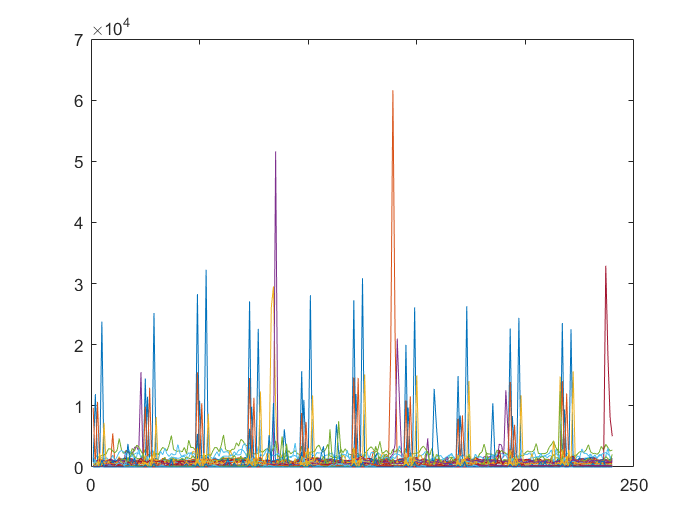
\includegraphics[scale=0.6]{offer.png}
    \caption{部分企业前五年的供货情况}     \label{fig:1}
\end{figure}

为了便于表述,后文中使用符号$X_1$、$X_2$、$X_3$和$X_4$来分别表示精确度的平均值、方差、供货总量与单次最大供货量这四个评价
指标。

\subsubsection{使用熵权法为指标客观赋权}
熵值法是一种根据各项指标指标值的变异程度来确定指标权数的客观赋权法。无论是选择$TOPSIS$法还是层次分析法,首先都需要得到评价指标的具体权重。$TOPSIS$法常常需要邀请专家对于评价指标打分,而层次
分析法则是通过两两比较各指标赋予其重要性标度来推算权重。这两种方法的弊病就是\textbf{赋权过程具有较大主观性},而基于客观数据信息量的
熵权法可以\textbf{基于指标的变异性大小客观赋权},很好的弥补了这一劣势。
%角标
\subsubsection*{熵权法的实现原理}
熵权法中的”熵“即信息熵,它指信息量的数学期望。这里的信息量是信息论中基于事物出现概率的概念
\begin{equation}
    I_i = log_2(\frac{1}{P_i})=-log_2P_i
    \label{信息量}
\end{equation}
由公式可见其与某事件出现的概率成反比。从意义上理解,信息量即将一个事物确定下来需要查询的信息的量。当某事物信息熵较小时,出现概率较大,
其就具有了较高的确定性(这意味着关于该事物的未知信息少,已知信息多),该事物所能提供的信息量就越大,那么它在综合评价体系中就具有了较大权重。
由其具有确定的计算公式,我们可以根据信息熵客观的为各个指标定量衡量权重。
\subsubsection*{熵权法赋权模型的建立与求解}
使用熵权法为指标客观赋权,我们首先将附录数据正向化,并进行了归一化处理
\begin{equation}
    Y_{ij}=\frac{X_{ij}-min(X_i)}{max(X_i)-min(X_i)}\large\nonumber
    \label{归一化}
\end{equation}
其中,对于$X_{ij}$,$i$取值介于$1\sim4$,表示四项评价指标。$j$取值介于$1\sim402$,表示各项指标对于每家供应商
的具体数据。由附表信息,$X_{ij}$的取值可以很容易得出。\par
利用正向标准化后的数据得到所有情况中各指标的比重(变异性),即前文所说的某事件出现的”概率“
\begin{equation}
    p_{ij}=\frac{Y_{ij}}{\sum_{i=1}^{n}{Y_{ij}}},i=1,\cdots,n,j=1,\cdots,m\nonumber
    \label{指标比重}
\end{equation}
将其代入信息熵的计算公式
\begin{equation}
    E_j = -\ln(n)^{-1}\sum_{i=1}^{n}{p_{ij}}\ln{p_{ij}}\nonumber
\end{equation}
这样就确定了对应于信息熵的已知信息量,各指标信息量的比重就客观反映了其权重
\begin{equation}
    w_j=\frac{1-E_j}{m-\sum E_j}(j=1,2,\cdots,m)
\end{equation}
\subsubsection*{熵权法程序设计}
值得注意的一点是,由于在实现熵权法的过程中,需要经过归一化、计算概率等相关处理,所以在实际程序编写的
过程中不可避免的会遇到概率值为0的情况。而在计算信息量时,由(1)式可知,其在0处没有定义。
(这是显而易见的,因为概率为零的信息量无穷大。所以在编程的过程中需要对归一化之后的数值经行修正,给其加上
一个很小的常数$\epsilon$\cite{黄鹏2015福建省土地生态安全AHP法和熵值法动态评价比较},从而使其有意义。\par
%%%%%%%%%%%%%%%%%%%%%%%%%%%%%%%%%%%%%%引用
熵权法为四个指标客观赋权的程序框图如下
\begin{figure}[H]
    \centering
    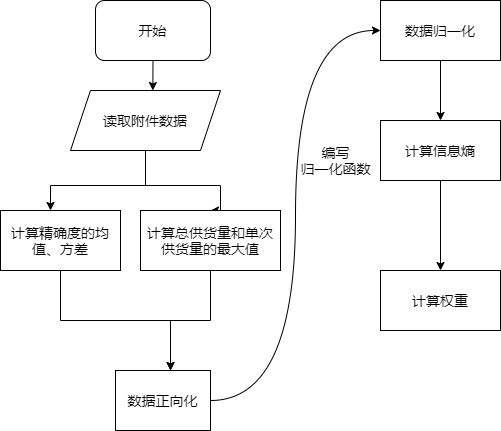
\includegraphics[scale=0.6]{shangquan.png}
    \caption{熵权法程序框图}     \label{fig:2}
\end{figure}
\subsubsection{结合TOPSIS法的综合评价}
\subsubsection*{TOPSIS法概述}
TOPSIS法(又称为”优劣解距离法“)是根据有限个评价对象与理想化目标的接近程度进行排序进而评价现有目标相对优劣
性的方法。其适用范围广泛,多应用于有量化指标的评价类问题上。其原理是检测评价对象对于”理想解“和”负理想解“
之间的距离,并以此为依据对各方案综合评分,排序确定评价对象的相对优劣。但其\textbf{缺点是权重值的得出通常具有主观性},导致
评价结果说服力不足。而此题\textbf{我们优化了TOPSIS评价模型,将其与熵权法结合,通过客观赋权增强其结论的说服力。}
\subsubsection*{TOPSIS法评价模型的建立}
对于有4个属性,402个评价对象的体系构建原始数据矩阵
\begin{equation}
    X=\begin{bmatrix}
        X_{11}   & X_{12}   & \dots  & X_{14}   \\
        X_{21}   & X_{22}   & \dots  & X_{24}   \\
        \vdots   & \vdots   & \ddots & \vdots   \\
        X_{4021} & X_{4022} & \dots  & X_{4024} \\
    \end{bmatrix} \quad
    \nonumber
    \label{数据矩阵}
\end{equation}
对该矩阵进行向量标准化处理,得到规范化矩阵$z$
\begin{equation}
    z_{ij}=\frac{X_{ij}}{\sqrt{\sum\limits^n_{i=1}X^2_{ij}}}\nonumber
    \label{规范化矩阵}
\end{equation}
结合$(1)$式熵权法确定的权重,构造加权规范化矩阵
\begin{equation}
    Z=(Z_{ij})_{(n\times m)}=z_{ij}\cdot w_j\nonumber
    \label{加权规范化矩阵}
\end{equation}
根据加权规范化矩阵,确定其”理想解“与”负理想解“
\begin{equation}
    Z^+ = (max\{Z_{11},Z{_21},\dots,Z_{n1}\},max\{Z_{12},Z_{22},\dots,Z_{n2}\},max\{Z_{1m},Z_{2m},\dots,Z_{nm}\}) =(Z^+_1,Z^+_2,\dots,Z^+_m)\nonumber
\end{equation}
\begin{equation}
    Z^+ = (min\{Z_{11},Z{_21},\dots,Z_{n1}\},min\{Z_{12},Z_{22},\dots,Z_{n2}\},min\{Z_{1m},Z_{2m},\dots,Z_{nm}\}) =(Z^-_1,Z^-_2,\dots,Z^-_m)\nonumber
\end{equation}
并以此计算最优、最劣距离
\begin{equation}
    D^+=\sqrt{\sum_{j=1}^{n}{(Z_{ij}-Z^+_j)^2}}\nonumber
\end{equation}
\begin{equation}
    D^-=\sqrt{\sum_{j=1}^{n}{(Z_{ij}-Z^-_j)^2}}\nonumber
\end{equation}
得到理想贴进度
\begin{equation}
    C_i=\frac{D^-_j}{D^+_j+D^-_j}\nonumber
\end{equation}
进行排序,选出前50名即为最重要的50家供货商。
\subsubsection*{TOPSIS法评价模型程序求解流程}
由于TOPSIS法中矩阵的规范化等价于正向化与归一化两个条件,因此我们编写程序时直接使用了熵权法已经处理过的正向归一化
矩阵以简化运算,程序流程如下:
\begin{description}
    \item[$\blacktriangleright$] \textbf{Step1} 读取规范化矩阵与权重表
    \item[$\blacktriangleright$] \textbf{Step2} 将规范化矩阵与熵权法得到的权重表运算得到加权规范化矩阵$Z$
    \item[$\blacktriangleright$] \textbf{Step3} 遍历$Z$得到“理想解“与”负理想解”
    \item[$\blacktriangleright$] \textbf{Step4} 计算最优、最劣距离并将结果排序
    \item[$\blacktriangleright$] \textbf{Step5} 输出前50名供货商
\end{description}
\newpage
\begin{description}
    \item[$\bigstar$] 结果展示:
\end{description}

\begin{longtable}{l|llll|l}
    \toprule
    编号 & 精确度平均值 & 精确度的方差 & 供货总量 & 单次最大供货量 & TOPSIS综合得分 \\
    \midrule
    140  & 1.199825272  & 0.160545743  & 302047   & 21293          & 0.675198902    \\
    348  & 1.070133152  & 0.09454509   & 92421    & 36972          & 0.622301599    \\
    151  & 0.983328206  & 0.020063101  & 194498   & 21267          & 0.564549137    \\
    201  & 0.536341199  & 0.254117575  & 81989    & 30977          & 0.563314813    \\
    229  & 0.994426055  & 0.004697454  & 354887   & 3147           & 0.480728969    \\
    361  & 0.992053674  & 0.005377459  & 328080   & 2816           & 0.458163546    \\
    374  & 1.312158559  & 0.112746088  & 49224    & 23695          & 0.446672752    \\
    108  & 0.984082869  & 0.01704667   & 240950   & 7885           & 0.423816598    \\
    139  & 1.243990587  & 0.097592391  & 151862   & 10207          & 0.343906103    \\
    330  & 0.985590135  & 0.019036115  & 136652   & 9768           & 0.319015574    \\
    126  & 0.989970416  & 0.186240219  & 47540    & 15114          & 0.312548133    \\
    308  & 0.974520012  & 0.028175881  & 136998   & 8181           & 0.297871994    \\
    282  & 1.013308551  & 0.004372127  & 169340   & 1724           & 0.279658746    \\
    340  & 0.999293707  & 0.001889266  & 171426   & 1181           & 0.279233345    \\
    275  & 1.003392888  & 0.000306742  & 158553   & 966            & 0.260688259    \\
    329  & 1.0019197    & 0.000537446  & 156518   & 971            & 0.257928479    \\
    307  & 1.244248204  & 0.16870653   & 78196    & 9385           & 0.241823064    \\
    131  & 0.997395498  & 0.009990159  & 137512   & 1014           & 0.231473631    \\
    356  & 1.002613641  & 0.005963545  & 130307   & 1788           & 0.225389591    \\
    268  & 1.00351123   & 0.000539785  & 129786   & 736            & 0.219065135    \\
    306  & 1.004597407  & 0.000568041  & 126096   & 922            & 0.214575308    \\
    395  & 0.918094209  & 0.120756485  & 75843    & 7661           & 0.2123179      \\
    194  & 1.00196034   & 0.001948659  & 101365   & 595            & 0.176387837    \\
    143  & 1.003667731  & 0.038807572  & 82787    & 2521           & 0.159062768    \\
    352  & 1.001534168  & 0.004841805  & 89031    & 699            & 0.157983582    \\
    37   & 1.14974634   & 0.158054432  & 50686    & 5398           & 0.147906884    \\
    247  & 1.013939114  & 0.000884787  & 56698    & 342            & 0.106691293    \\
    284  & 1.0381543    & 0.002036033  & 46597    & 2005           & 0.101056396    \\
    365  & 1.021696663  & 0.002089781  & 41631    & 381            & 0.083795136    \\
    31   & 1.019774282  & 0.003261046  & 41207    & 251            & 0.082807204    \\
    338  & 1.264371563  & 0.111733709  & 30109    & 2081           & 0.076270086    \\
    40   & 1.018751142  & 0.01216166   & 31905    & 432            & 0.069710381    \\
    364  & 1.038518536  & 0.009651035  & 28763    & 618            & 0.065988507    \\
    55   & 1.039824474  & 0.040958131  & 24041    & 1216           & 0.063155977    \\
    367  & 1.030694449  & 0.022426908  & 26335    & 597            & 0.062481832    \\
    346  & 1.016227876  & 0.017439483  & 23240    & 162            & 0.057352717    \\
    294  & 1.042035369  & 0.00644309   & 18842    & 113            & 0.051993084    \\
    86   & 1.195310114  & 0.179352469  & 17949    & 1265           & 0.051884414    \\
    80   & 1.086134053  & 0.040086494  & 19237    & 215            & 0.051179135    \\
    244  & 1.071080527  & 0.046899012  & 16406    & 180            & 0.047954646    \\
    218  & 1.098141397  & 0.024692137  & 15483    & 180            & 0.047237803    \\
    74   & 1.006205778  & 0.232847768  & 13051    & 1043           & 0.046185824    \\
    210  & 0.832213153  & 0.241177511  & 15694    & 1034           & 0.046177575    \\
    3    & 1.059890496  & 0.113518145  & 13138    & 387            & 0.043638188    \\
    114  & 1.168151472  & 0.116036871  & 10931    & 721            & 0.041843506    \\
    273  & 0.993120594  & 0.135664811  & 9484     & 537            & 0.041576485    \\
    189  & 1.016986759  & 0.086221784  & 8892     & 116            & 0.04083377     \\
    78   & 0.990774338  & 0.122525234  & 8553     & 412            & 0.040602391    \\
    5    & 1.04055103   & 0.09553314   & 6912     & 128            & 0.038895059    \\
    291  & 1.149152262  & 0.14595773   & 7984     & 686            & 0.038785968    \\
    \bottomrule
\end{longtable}

\subsubsection{结合层次分析法的综合评价}

\subsubsection*{层次分析法概述}
层次分析法是一种分层次的权重决策分析方法,善于将定性问题定量化。其本质是用分层分析的思想将多目标决策问题拆解为多个影响因素之间的
定量分析。本题中评价供货商重要与否就同样可以使用层次分析法的思考方式。在此基础上,我们结合了熵权法得出的指标权重,且由于已知各项指标的具体数据
已知,我们省去了层次分析法中两两比较主观赋权的过程,而是利用客观数据反映判断矩阵的标度值,极大的避免了层次分析法的盲目性与不确定性。
此方法也可以为TOPSIS法的结果作出印证。
\subsubsection*{层次分析法模型的建立与求解}
\begin{description}
    \item[$\blacktriangleright$] \textbf{建立层次结构}\par
        按层次分析法将决策系统自上而下分为目标层、准则层与方案层三个层次,层次结构如图所示:
        \begin{figure}[htbp]
            \centering
            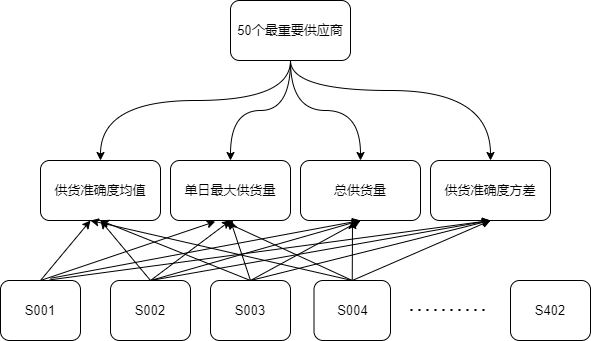
\includegraphics[scale=0.6]{AHP.png}
            \caption{层次分析法示意图}     \label{fig:3}
        \end{figure}
        \\
        \\
    \item[$\blacktriangleright$] \textbf{构造判别矩阵}\par
        对于各项指标的权重关系,我们采用了熵权法的结果,避免了赋权的主观性。而确定各指标对于供应商的权重时,我们选择采用算术平均、几何平均与特征值法三种方法综合,对
        前面计算中得到的各项指标的客观数据求权重,同样避免了主观赋权对于真实结果的影响。\par
        综合每一个供货商关于所有指标的计算结果,得到最终的权重矩阵\par
        \begin{table}[htbp]
            \begin{tabular}{|l|l|l|l|l|}
                \hline
                                         & 指标权重    & S001        & S002        & ...      \\
                \hline
                准确度均值               & 0.01915795  & 0.337362637 & 0.919749373 & $\cdots$ \\
                \hline
                准确度方差               & 0.021462962 & 0.381477411 & 0.433076045 & $\cdots$ \\
                \hline
                总供货量                 & 0.438240822 & 49          & 273         & $\cdots$ \\
                \hline
                准确度均值单日最大供货量 & 0.521138266 & 6           & 67          & $\cdots$ \\
                \hline
            \end{tabular}
        \end{table}
        将供应商各项权重列与指标权重列一一对应相乘并求和,得到基于熵权法与层次分析法评价体系的供货商最终得分。

    \item[$\bigstar$] 层分析法求解结果展示:
        \begin{longtable}{l|llll|l}
            \toprule
            编号 & 精确度平均值 & 精确度的方差 & 供货总量 & 单次最大供货量 & TOPSIS综合得分 \\
            \midrule
            140  & 1.199825272  & 0.160545743  & 302047   & 21293          & 0.704336915    \\
            348  & 1.070133152  & 0.09454509   & 92421    & 36972          & 0.671265896    \\
            151  & 0.983328206  & 0.020063101  & 194498   & 21267          & 0.579546338    \\
            201  & 0.536341199  & 0.254117575  & 81989    & 30977          & 0.560696564    \\
            229  & 0.994426055  & 0.004697454  & 354887   & 3147           & 0.522947876    \\
            361  & 0.992053674  & 0.005377459  & 328080   & 2816           & 0.485106422    \\
            108  & 0.984082869  & 0.01704667   & 240950   & 7885           & 0.448400194    \\
            374  & 1.312158559  & 0.112746088  & 49224    & 23695          & 0.425390897    \\
            139  & 1.243990587  & 0.097592391  & 151862   & 10207          & 0.36387778     \\
            330  & 0.985590135  & 0.019036115  & 136652   & 9768           & 0.346099315    \\
            308  & 0.974520012  & 0.028175881  & 136998   & 8181           & 0.32362686     \\
            126  & 0.989970416  & 0.186240219  & 47540    & 15114          & 0.305781555    \\
            282  & 1.013308551  & 0.004372127  & 169340   & 1724           & 0.273603295    \\
            340  & 0.999293707  & 0.001889266  & 171426   & 1181           & 0.268857797    \\
            307  & 1.244248204  & 0.16870653   & 78196    & 9385           & 0.258882151    \\
            275  & 1.003392888  & 0.000306742  & 158553   & 966            & 0.249930644    \\
            329  & 1.0019197    & 0.000537446  & 156518   & 971            & 0.247509025    \\
            395  & 0.918094209  & 0.120756485  & 75843    & 7661           & 0.236502238    \\
            356  & 1.002613641  & 0.005963545  & 130307   & 1788           & 0.226456584    \\
            131  & 0.997395498  & 0.009990159  & 137512   & 1014           & 0.224307037    \\
            268  & 1.00351123   & 0.000539785  & 129786   & 736            & 0.211151881    \\
            306  & 1.004597407  & 0.000568041  & 126096   & 922            & 0.209194359    \\
            143  & 1.003667731  & 0.038807572  & 82787    & 2521           & 0.176960759    \\
            194  & 1.00196034   & 0.001948659  & 101365   & 595            & 0.174047598    \\
            37   & 1.14974634   & 0.158054432  & 50686    & 5398           & 0.170928484    \\
            352  & 1.001534168  & 0.004841805  & 89031    & 699            & 0.160191009    \\
            284  & 1.0381543    & 0.002036033  & 46597    & 2005           & 0.125571674    \\
            247  & 1.013939114  & 0.000884787  & 56698    & 342            & 0.115119818    \\
            338  & 1.264371563  & 0.111733709  & 30109    & 2081           & 0.098089909    \\
            365  & 1.021696663  & 0.002089781  & 41631    & 381            & 0.096868662    \\
            31   & 1.019774282  & 0.003261046  & 41207    & 251            & 0.094510349    \\
            40   & 1.018751142  & 0.01216166   & 31905    & 432            & 0.085290168    \\
            55   & 1.039824474  & 0.040958131  & 24041    & 1216           & 0.085232121    \\
            364  & 1.038518536  & 0.009651035  & 28763    & 618            & 0.083729036    \\
            367  & 1.030694449  & 0.022426908  & 26335    & 597            & 0.08015199     \\
            346  & 1.016227876  & 0.017439483  & 23240    & 162            & 0.070652613    \\
            86   & 1.195310114  & 0.179352469  & 17949    & 1265           & 0.070618444    \\
            294  & 1.042035369  & 0.00644309   & 18842    & 113            & 0.064398908    \\
            80   & 1.086134053  & 0.040086494  & 19237    & 215            & 0.064309174    \\
            74   & 1.006205778  & 0.232847768  & 13051    & 1043           & 0.063329308    \\
            210  & 0.832213153  & 0.241177511  & 15694    & 1034           & 0.063007103    \\
            244  & 1.071080527  & 0.046899012  & 16406    & 180            & 0.060382775    \\
            218  & 1.098141397  & 0.024692137  & 15483    & 180            & 0.059469472    \\
            3    & 1.059890496  & 0.113518145  & 13138    & 387            & 0.057209759    \\
            114  & 1.168151472  & 0.116036871  & 10931    & 721            & 0.056978949    \\
            273  & 0.993120594  & 0.135664811  & 9484     & 537            & 0.055096933    \\
            78   & 0.990774338  & 0.122525234  & 8553     & 412            & 0.052587767    \\
            291  & 1.149152262  & 0.14595773   & 7984     & 686            & 0.052197741    \\
            189  & 1.016986759  & 0.086221784  & 8892     & 116            & 0.049921203    \\
            5    & 1.04055103   & 0.09553314   & 6912     & 128            & 0.046864135    \\
            \bottomrule
        \end{longtable}
\end{description}

\subsection{问题二模型的建立与求解}
\subsubsection{供货商范围的确定}
 首先出于将复杂问题拆解为小问题的考虑,其次也是为之后的动态规划计算做铺垫,我们首先使用了
贪心算法和0-1规划对50个重要供货商进一步排序使得他们更加契合本问的要求。
\subsubsection*{贪心算法}
\begin{description}
    \item[$\blacktriangleright$] \textbf{贪心算法概述}\par
对于一个具有最优子结构的问题,可以对其使用贪心算法求解。结合熵权法分析得出,供应商的供货能力是影响其评价体系的主要因素。对于此问题,如果以过去五年的平均供货量作衡量供应商
对厂商生产需求的重要程度的指标,任意供应商$A,B$的平均供货量在排序交换之后是没有变化的,这时我们也称
以平均供货量作为评价标准下,选择供应商具有最优子结构。此时只需要贪心地根据平均供货量从大到小选择供应商即可。但
要注意的是,在求解平均供货量数据中由于厂家未下订单的数据不具参考价值,应当剔除!
\item[$\blacktriangleright$] \textbf{贪心算法程序设计}\par
如图\ref{fig:4}所示,贪心算法主要由判断、计算、得出结果三部分组成。其中的计算与得出结果都比较容易。
而判断是否具有最优子结构往往是不容易想到的,此题中供货商之间的平均供货量彼此无关且顺序不影响指标,所以其为最优子结构。
\begin{figure}[H]
    \centering
    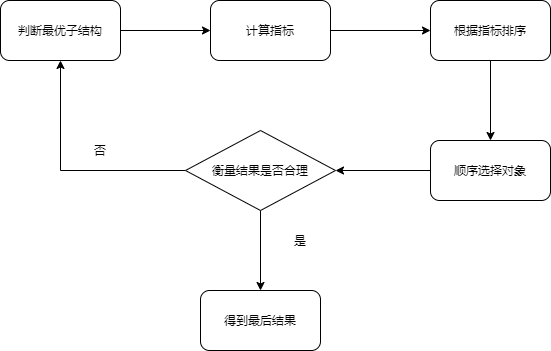
\includegraphics[scale = 0.6]{test.png}
    \centering
    \caption{贪心算法流程} \label{fig:4}
\end{figure}

\end{description}
\subsubsection*{0-1规划}


\subsection{问题三模型的建立与求解}
\subsection{问题四模型的建立与求解}
\section{模型的分析与检验}
\subsection{问题一结果的分析与检验}
对于问题一,可以通过对比两种算法的运行结果来检验得到结果的正确性。通过对比两个五十家重要供应商名单的列表,容易发现:结合了熵权法的TOPSIS法与层次分析法得到的结果无论是涵盖的供应商还是其排列序号都几乎
吻合。两种不同评价方式得出几乎一致的结果,说明二者互相佐证了结论的正确性\par
此外,我们使用本问确定的四项评价指标对全部402家企业进行了\textbf{聚类分析},由图可以发现
\begin{figure}[htbp]
    \centering
    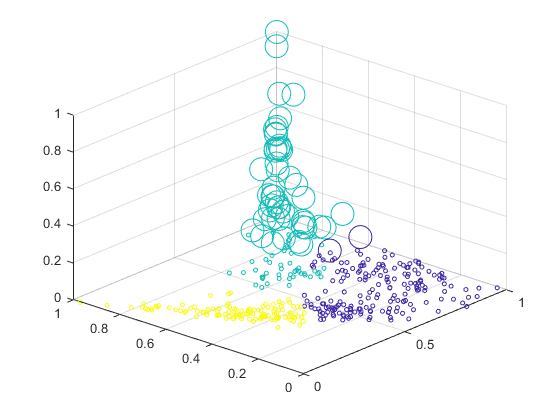
\includegraphics[scale = 0.7]{julei.png}
    \centering
    \caption{聚类分析结果,图中圆圈为结果名单中的50家重要企业} \label{fig:5}
\end{figure}
其中竖直方向的坐标轴表示企业供货能力大小,水平方向两条轴表示供货精确度。可以发现,位列50家重要供应商名单中的企业几乎全部被聚类算法划分到了“具有较强供货能力”一类,
而根据本道题其他问的分析与熵权法客观赋权得到的结果都可以说明供货能力是评价供应商对企业重要程度的最主要因素,名单企业几乎均位列此类,充分说明了问题一求解结果的合理性。
\subsection{问题二结果的分析与检验}
\subsection{问题三结果的分析与检验}
\subsection{问题四结果的分析与检验}

\section{模型的评价、改进与推广}
\begin{description}
\item[$\blacktriangleright$] 第二问中贪心法的使用虽然可以较容易的对平均供货量做出衡量,但是实际考虑制定满足企业生产的方案时不只有平均供货量这一个评判指标,故单纯考虑贪心法具有一定局限性,还需要综合考虑其他计算方法。
\end{description}

%参考文献
\bibliographystyle{plain}
\bibliography{reference}
\newpage
%附录
\begin{appendices}
\section{熵权法--matlab程序}
\subsection{将生产三种原料企业的产能转化为同类型}
\begin{lstlisting}[language=matlab]
filename = '附件1 近5年402家供应商的相关数据.xlsx';
providesheet = '供应商的供货量(m³)';

[power, text] = xlsread(filename,providesheet);
text = text(2:403,2);

for i = 1:402
    divnum = 0;
    if char(text(i)) == 'A'
        divnum = 0.6;
    elseif char(text(i)) == 'B'
        divnum = 0.66;
    else
        divnum =0.72;
    end
    power(i,:) = power(i,:)./divnum;
end

xlswrite('转化产能表.xlsx',power);
    \end{lstlisting}
\begin{lstlisting}[language=matlab]
filename = '转化产能表.xlsx';
ordersheet = '企业的订货量(m³)';
providesheet = '供应商的供货量(m³)';

%读入数据
order = xlsread(filename,ordersheet);
provide = xlsread(filename,providesheet);

%计算同步率方差和均值
meanratio = [];
varratio = [];
for i = 1:402
  campany = order(i,:);
  provider = provide(i,:);
  ratio = provider./campany;
  numberIndex = find(~isnan(ratio));
  ratio = ratio(numberIndex);
  meanratio = [meanratio, mean(ratio)];
  varratio = [varratio, var(ratio)];
end

%计算总供货量和和单次供货最大值
sumorder = sum(provide, 2);
maxorder = max(provide,[], 2);
xlswrite('指标.xlsx',[meanratio', varratio', sumorder, maxorder]);



%正向化归一化
meanratio = 1 - abs(meanratio - 1)/max(abs(meanratio - 1));
meanratio = unify(meanratio);
meanratio = handleZero(meanratio);

varratio = max(varratio) - varratio;
varratio = unify(varratio);
varratio = handleZero(varratio);

sumorder = unify(sumorder);
sumorder = handleZero(sumorder);

maxorder = unify(maxorder);
maxorder = handleZero(maxorder);

indexMatrix = [meanratio', varratio', sumorder, maxorder];
xlswrite('标准化矩阵和权重.xlsx',indexMatrix,'归一矩阵');

%计算信息熵
for i = 1:4
  line = indexMatrix(:,i);
  line = line ./ sum(line);
  indexMatrix(:,i) = line;
end
E = - (sum(indexMatrix .* log(indexMatrix)))/log(402);

%计算权重
w = (1 - E)/(4 - sum(E));
xlswrite('标准化矩阵和权重.xlsx',w,'权重');

%定义归一化函数
function ret = unify(array)
  ret = (array - min(array))/(max(array) - min(array));
end
function ret = handleZero(array)
  array(find(array == 0)) = 0.00001;
  ret = array;
end
 \end{lstlisting}
 \section{TOPSIS法--matlab程序}
 \begin{lstlisting}[language=matlab]
%W,P 需要导入w(4X1)p(402X4)两个矩阵
clear;

%计算加权规范化矩阵
p = xlsread("标准化矩阵和权重 (1)","归一矩阵");
w = xlsread("标准化矩阵和权重 (1)","权重");
index = xlsread("指标 (1)","sheet1");
Z = zeros(402,4);
for i =1:402
    for j =1:4
        Z(i,j) = p(i,j)*w(j);
    end
end

%通过遍历得到“理想解”与“负理想解”
best =[0,0,0,0];
worst=[1,1,1,1];
[r,c] = size(p);
for j =1:c
    for i =1:r
        if Z(i,j)>best(j)
            best(j) = Z(i,j);
        end
        if Z(i,j)<worst(j)
            worst(j) = Z(i,j);
        end
    end
end

%计算最优、最劣距离
[r,c] = size(Z);
Dplus = zeros(402,1);
Dsub = zeros(402,1);
for i = 1:r
    for j = 1:c
        Dplus(i) = Dplus(i)+ (Z(i,j)-best(j))^2;
        Dsub(i) = Dsub(i)+(Z(i,j)-worst(j))^2;
    end
end
for i =1:r
        Dplus(i) = sqrt(Dplus(i));
        Dsub(i) =sqrt(Dsub(i));      
end

%得到理想贴进度
C = zeros(402,1);
for i = 1:402
    C(i) = Dsub(i)/(Dplus(i) + Dsub(i));
end

%将结果排序并输出前50名
[A,postion] = sort(C);
temp = flipud(postion);
paiming =temp(1:50);
temp = [paiming,index(paiming,:),C(paiming,:)];
xlswrite("结果排名",temp,"sheet1");
\end{lstlisting}
\section{层次分析法--matlab程序}
\begin{lstlisting}[language=matlab]
%读入数据
filename = '标准化矩阵和权重.xlsx';
matrixsheet = '归一矩阵';
weightsheet = '权重';

matrix = xlsread(filename,matrixsheet);
weight = xlsread(filename,weightsheet);
zhi = xlsread('指标.xlsx');

%得到加权规范化矩阵
score = weight * matrix';

%计算综合得分并输出前50名
[sortedScore, I] = sort(score);
top50 = flipud(I');
top50 = top50(1:50);
xlswrite('AHP结果.xlsx',[top50, zhi(top50,:),score(top50)']);
\end{lstlisting}
\end{appendices}
\end{document}